\chapter{差分隐私策略机制的均衡优化模型}\label{chapter06}
{\em 本章针对差分隐私存在策略型攻击问题,基于差分隐私通信模型,提出隐私保护的攻防博弈模型,以实现隐私保护的隐私与数据效用均衡。首先,定义差分隐私保护系统中隐私保护者与攻击者(敌手)的隐私目标,并将其表述为隐私泄露的极大极小问题。针对该问题,以隐私度量为效用函数,构建两方零和对策博弈模型,并基于极大极小定理、凹凸博弈给出相应的博弈均衡分析。理论分析表明鞍点的存在,并进一步给出鞍点的内涵。其次,对于等价的$\epsilon$- 隐私机制,提出等价类隐私机制可比较的方法,解决$\epsilon$-隐私度量存在的不足。最后,基于交替最优响应设计鞍点计算的策略优化选择算法。理论分析及实验结果表明提出的方法可辅助隐私保护者评估隐私泄露风险。}
\section{引言}
近年来,私有敏感信息泄露问题引起了社会和学术研究领域的广泛关注,正在成为大数据时代的一个主要挑战。如医疗数据、在线社交活动、基于位置的服务等网络应用中对个人数据的使用,使得个人的隐私遭受到了潜在的风险,由此产生了用户隐私泄露问题。隐私泄露逐渐成为数据收集、发布、分析、感知等隐私计算\cite{Lifenghua16}任务中迫切需要解决的问题,技术层面上亟需有效的隐私保护模型与算法。围绕隐私保护的核心任务,学术研究已提出诸多的隐私保护模型及解决方案。其中,差分隐私\cite{dwork2006differential,dwork2006calibrating,dwork2014algorithmic}是广泛被接受的隐私保护模型。为了克服基本假设中存在可信实体的局限性,本地模型的差分隐私\cite{duchi2013local,duchi2013Minimax}(Local Differential Privacy,LDP)被提出,并主要应用于解决数据收集阶段的隐私保护问题。在差分隐私的本地模型中,每一个用户独立的扰动自己的原始数据,然后报告扰动后的数据给数据聚合者(收集者)。由于本地模型的显著特性,一经提出就受到学术研究和产业应用的关注。学术界围绕本地模型的应用,先后提出诸如RAPPOR\cite{fanti2016building,erlingsson2014rappor}、$k$-RR\cite{kairouz2016extremal}、OUE\cite{wang2017locally}等众多著名先进的隐私机制。产业界如Google Chrome 浏览器\cite{erlingsson2014rappor}、Apple公司操作系统\cite{tang2017privacy}等将其应用于隐私保护数据收集、分析场景。纵观研究工作,数据聚合者通常是半诚实的敌手模型,隐私性与数据质量依然是核心的关注问题,隐私保护难以实现完美无泄露,相对的寻找隐私保护策略均衡成为较为理想的权衡折中解决方案。

实际的应用中,随机化响应\cite{warner1965randomized}技术是有效实现LDP的方法\cite{kairouz2016extremal,kairouz2016discrete,wang2016using,holohan2017optimal},其已成为LDP方案设计的基本构建模块。本质上,随机化响应是从原始数据到扰动输出数据的一个概率性映射。基于此,隐私机制的随机性与隐私保护的隐私和数据质量密切相关,这就是权衡隐私与效用课题的研究内容。目前,这仍然是差分隐私保护中学术研究的重点。在差分隐私本地模型的数据收集应用中,数据聚合者收集、存储、分析用户报告的扰动数据\cite{sei2017differential},扰动后的数据与原始数据之间的关联决定了隐私保护的隐私性与数据的可用性。为了解决权衡的问题,在寻找有效的折中方案过程中,隐私与数据质量的度量是基本的前提工作。当前,隐私预算参数$\epsilon$是一个量化差分隐私不可区分等级的事实标准。但是,这个度量是分布独立的,其存在着一些不足之处。例如,一个确定性的隐私协议$Q(x)=x$ mod $2$提供$\epsilon = \infty$的隐私保障,但是该隐私协议仍然可以阻止部分的隐私泄露\cite{lopuhaa-zwakenberg2019information}。除了上面提到的,这样的隐私度量无法在等价的$\epsilon$-隐私机制集合中区分那个隐私机制的性能更好,因为集合中的隐私机制都提供相同的$\epsilon$-不可区分等级。受这些问题的激励,度量也亟需新的评价方法。

针对上述问题,从隐私信息流的角度,基于信息论的方法可以得到有效的解决\cite{wu2020a}。首先,上述有关LDP机制的数据处理过程,可以被建模为一个原始数据与扰动数据之间的噪声信道模型\cite{xiong2016randomized,kalantari2018robust}(参见\ref{sec:communication_model_of_dp}节内容)。然后,利用熵与互信息量定义隐私泄露度量,且已在诸多研究工作中得到了应用\cite{kairouz2016extremal,calmon2012privacy,sarwate2014a,kalantari2016optimal}。重要的,信息论的模型中考虑了数据分布和隐私机制对隐私泄露的影响,互信息隐私测量扰动数据包含原始数据的信息量,它捕捉住了隐私攻击者有关数据分布的先验知识。此外,隐私保护系统中仅有两方的参与者\cite{dwork2014algorithmic},用户本地执行隐私协议旨在减少隐私泄露,其类似于隐私防护者。相似的,聚合者试图最大化隐私泄露,以至于推断用户的个人信息,类似于隐私攻击者。鉴于上述分析,本章中关注的问题演变为了有关隐私的攻防对抗问题。自然的,以博弈均衡的思想解决这个问题不失为一个理想的选择。现有存在的工作中,二人零和对策博弈\cite{hsu2013differential,alvim2017information,alvim2018leakage,jin2019on}、斯坦伯格博弈\cite{fioretto2020differential}、贝叶斯博弈\cite{cui2019improving}等在差分隐私框架下都有一定的应用。重要的,从量化信息流的角度构建的信息泄露博弈\cite{alvim2017information,alvim2018leakage}、量化信息流博弈\cite{jin2019on}是有效的隐私分析方法。


鉴于上述的分析,本章中考虑在理性的框架下使用信息论的方法解决隐私与效用的均衡问题,通过分析隐私保护者与攻击者的隐私目标,首先将其形式化表述为隐私的极大极小问题。然后,基于差分隐私通信模型(\ref{sec:communication_model_of_dp}节),提出隐私保护的攻防博弈模型,也即是一个二人的零和博弈模型。进一步,提出一个交替最优化算法计算提出的攻防博弈的鞍点,利用鞍点策略实现差分隐私的均衡优化。理论上的均衡分析和实验结果表明,提出的均衡思想是一种稳定的状态,可用于预测评估隐私泄露风险。本章的主要贡献可以总结如下:

(1) 通过使用信息论的方法量化隐私攻击者的信息增益,提出了隐私保护的攻防博弈模型(PPAD),用于分析用户和聚合者的理性策略行为。
	
(2) 在隐私与效用的原则下,分析隐私防护者与攻击者的隐私目标,形式化表述互信息隐私的极大极小问题,构建二人零和对策博弈求解形式化表述的极大极小问题,并利用交替最优响应策略,设计交替最优的策略优化选择算法。
	
(3) 对于等价的$\epsilon$-隐私机制,提出一种有效的比较分析方法,并进一步验证了互信息隐私泄露在最差情况下可以达到隐私泄露的上界,为隐私泄露风险评估提供了量化分析的方法。


本章其余部分组织如下:首先,第\ref{sec:chapter06-system-model}节阐述本章的系统模型、敌手模型,提出研究问题。其次,第\ref{sec:chapter06-PPAD}节提出隐私保护的攻防博弈模型(PPAD),并给出均衡分析。进一步,第\ref{sec:chapter06-algorithm}节介绍均衡求解的策略优化选择算法。最后,第\ref{sec:chapter06-experiment}节给出实验与分析,并在第\ref{sec:chapter06-conclusion}节总结本章的研究工作。

\section{系统模型与问题提出}\label{sec:chapter06-system-model}
本节首先介绍本章的系统模型与符号表示,随后,阐述敌手攻击模型并给出问题描述及形式化表述。
\subsection{系统模型}
如图~\ref{Fig:chapter07_architecture}描绘了本章的系统模型,其中包含一个不可信数据聚合者和诸多的用户参与到系统数据处理流程中,并通过网络实现互联。本章中重点关注于系统中的隐私保护问题,因此忽略具体的内部网络连接细节。为了保护用户的隐私,每个用户独立的执行隐私保护协议扰动其自己的私密数据。本章中假设用户执行相同的隐私协议,并且隐私协议由用户和聚合者共同协商决定。在这样的情景下,隐私保护的数据处理遵循以下的三个步骤。
\begin{figure}[!ht]
	\centering 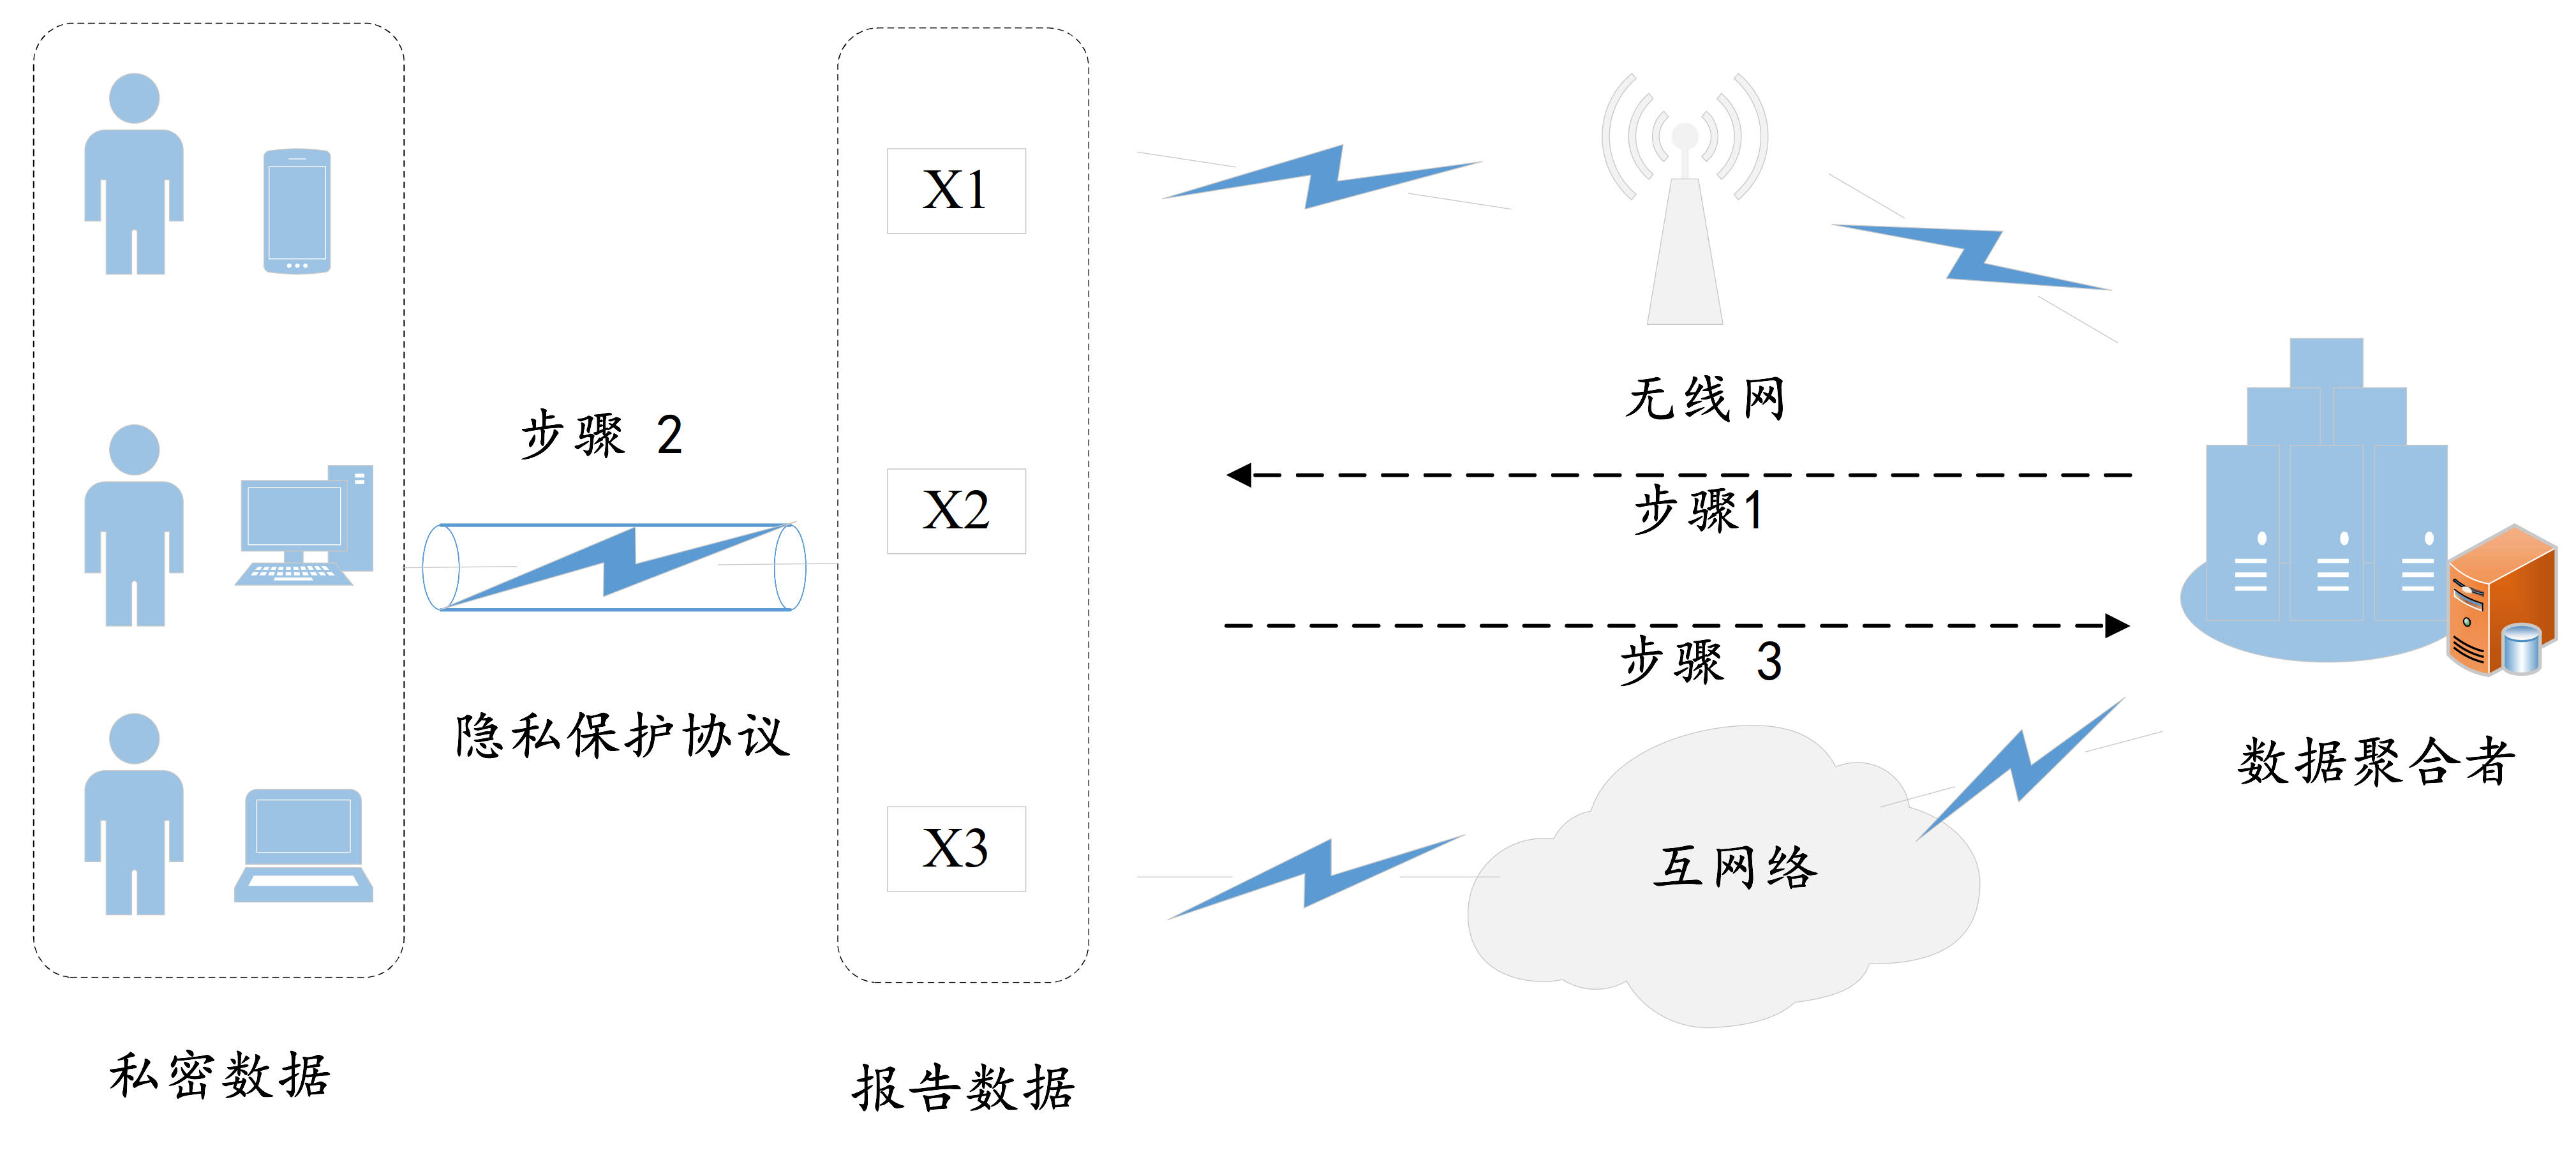
\includegraphics[width=5.5in,height=2.5in]{./figures/Application_architecture.jpg}
	\caption{隐私保护数据收集的系统模型}
	\label{Fig:chapter07_architecture}
\end{figure}

步骤1: 数据聚合者发布一个数据收集的信号,并决定收集数据的具体细节。这些将要被收集的数据可能包含个人的数据,如家庭地址、婚姻状态、性别、年龄等。然后,数据聚合者招募用户去上报她们自己的私密数据。

步骤2: 系统中的用户可以决定是否上报他们的数据给数据聚合者。如果一个用户同意参与到当前的数据收集任务,她将执行隐私保护协议得到伪装的数据,然后将得到的伪装数据上报给数据聚合者。

步骤3: 基于上述步骤1和步骤2,数据聚合者收集、存储用户的上报数据,然后分析这些上报的数据。


针对图~\ref{Fig:chapter07_architecture}描述的隐私保护数据收集系统模型,假设有$n$个用户参与,$[n]=\{1,2,\cdots,n\}$。有限集合$\mathcal{X}$和$\hat{\mathcal{X}}$分别表示用户数据和伪装数据的所有可能取值域,进一步,$|\mathcal{X}|$表示有限集合$\mathcal{X}$的不同原子数量,使用从$1$到$|\mathcal{X}|$的整数几个表示$\mathcal{X}$中真实字母表的序数。离散随机变量$X$和$\hat{X}$分别表示个人的原始数据和伪装数据。由此,LDP形成一个概率性函数,映射$x \in \mathcal{X}$到$\hat{x} \in \hat{\mathcal{X}}$的概率为$Q(\hat{x}|x)$,记作,$Q:\mathcal{X}\rightarrow \hat{\mathcal{X}}$。除此之外,本章中有时使用下标的$x_i$和$\hat{x}_i$表示第$i$个用户的数据和伪装数据。

为了保护用户个体的隐私信息,每个用户独立的扰动自己的原始数据得到扰动的数据,然后将扰动数据发送给数据聚合者。不失一般性,混淆机制与噪声信道相关,因为差分隐私的定义是基于一个随机的概率性函数。通过这种方式,LDP与信息论建立了基本的联系。为了更好的说明这种关系,以下给出一个具体的例子。

\begin{example}对于``是''和``否''的选择型问题,它可以被$\{0,1\}$二进制的候选集表示。对于这类问题,差分隐私的混淆机制可以被视为一个二元对称信道。例如,$Q_{0|0}=Q_{(1|1)}=0.7$和$Q_{010}=Q_{(0|1)}=0.3$,则其满足$\epsilon=\ln \frac{7}{3}$的$\epsilon$-差分隐私。
\end{example}

令$P$是支撑集$\mathcal{X}$上的任意一个概率分布,有限集合$\mathcal{P}$包含$\mathcal{X}$上所有可能的概率分布,则有$P\in \mathcal{P}$。 假设每一个用户的个人私密数据独立地抽样于的一个分布$P\in \mathcal{P}$,数据聚合者不知道这个分布$P$,仅知道它是集合$\mathcal{P}$的元素。基于这样的模型假定,本章中考虑策略型的敌手和数据聚合者知道彼此的策略空间。在这种情况下,聚合者旨在最大化隐私推断的成功概率。
\subsection{敌手模型}\label{adversary:model}

本章中,攻击模型是一个半诚实但好奇的(Semi-honest-but curious)敌手模型,也就是,数据聚合者诚实的执行隐私保护协议,但是试图从用户报告的扰动数据中去推断用户的个人隐私信息。事实上,聚合者可能是一个消息灵通的策略型敌手,他可能知道一些有关数据分布的先验知识帮助推断用户隐私。为了捕捉这个先验,假设聚合者仅知道数据分布属于一个确定的集合,$P\in \mathcal{P}$,但是不知道确切的数据分布$P$。在此情况下,本章中考虑一个策略型的敌手$A$,他知道用户的隐私保护策略集$\mathcal{Q}$,并有一些数据分布的先验知识$\mathcal{P}$,目标是获取最大的隐私信息量以保证能够推断、识别用户的真实隐私信息。

\subsection{问题提出}\label{sec:chapter06-problem}
差分隐私的预算参数$\epsilon$是量化隐私保护不可区分等级的事实标准,但是,$\epsilon$-度量提供了最差情况下的隐私保证,那也就是说,这个度量是对隐私攻击者有一个较强的假设。因为$\epsilon$-度量仅依赖于概率性映射函数,如引言中所述的这个度量存在着一些不足之处\cite{lopuhaa-zwakenberg2019information}。如果存在一个隐私保护机制集合$\mathcal{Q}$,集合中的每个元素$Q\in \mathcal{Q}$都提供$\epsilon$-隐私保障,则$\epsilon$-度量无法区分哪一个机制具有较好的隐私保护效果。然而,在很多的应用中,这些隐私保护机制的质量又迫切需要评估。针对这个问题,信息论方法提供了一种有效的解决途径,以下从定义开始介绍其方法的具体细节。

\begin{definition}\label{def:equivalent_privacy_mechanism}离散有限集合$\mathcal{Q}$表示一个含有$k$个隐私保护机制的集合。如果$\mathcal{Q}$中的每一个机制$Q^i:\mathcal{X}\rightarrow\hat{\mathcal{X}}$(s.t.$1\leq i \leq k$)是一个$\epsilon$-隐私机制,则这些机制$\{Q^i\}_{i=1}^{k}$称为一个等价$\epsilon$-隐私机制。
	
\end{definition}
\begin{remark}{\em 上述定义}\ref{def:equivalent_privacy_mechanism}{\em 可以被放松获得一个宽松的LDP机制集合,也就是,一个任意的隐私机制$Q^i \in \mathcal{Q}$是$\epsilon_i$-LDP机制。}
\end{remark}


事实上,隐私保护机制$Q^i:\mathcal{X}\rightarrow\hat{\mathcal{X}}$是一个损失压缩机制,它控制着从原始数据到伪装数据的隐私信息比特流动。为了量化信息的流动量,使用信息论的方法定义聚合者的信息增益为
\begin{definition}\label{def:information_gain}
	对于给定的隐私信息$x_i$,概率分布$P(X=x_i)$和$P(X=x_i|\hat{X}=\hat{x}_i)$分别表示先验分布和观察到$\hat{x}_i$后的后验概率分布。概率分布的比值$\log\left(\frac{P(X=x_i|\hat{X}=\hat{x}_i)}{P(X=x_i)}\right)$定义为聚合者的信息增益。
\end{definition}

基于上述定义\ref{def:information_gain},可以在观察到扰动数据之后,测量有关原始数据的不确定度减少量。本质上,这个度量是关于原始数据的先验和后验概率分布的比较。此外,注意到这个度量和信息论中著名的互信息具有相同的形式。重要地,期望形式的互信息测量一个用户的平均信息损失量,可以用来测量隐私机制的隐私泄露量,也就是互信息泄露
\begin{equation}
	I(X;\hat{X})=\sum_{x\in\mathcal{X}}\sum_{y\in\hat{\mathcal{X}}}P(x)Q(\hat{x}|x)\log\left(\frac{Q(\hat{x}|x)}{P(y)}\right)
\end{equation}
基于互信息隐私泄露的概念,等价的$\epsilon$隐私机制之间是彼此可以比较的。为了阐述一个偏序关系,首先给出以下定义
\begin{definition}
	对于一个给定的先验概率分布$P$,和任意的两个隐私机制$Q^i,Q^j\in \mathcal{Q}$(s.t.$1\leq i,j\leq k$)。如果$I(P;Q^i)\leq I(P;Q^j)$,则有$Q^i\succcurlyeq Q^j$;否则,$Q^i \prec Q^j$。
\end{definition}

具体的来说,这种偏序关系是可以传递的,它可以用来比较不同机制的隐私保护强度。接下来,考虑互信息测量隐私泄露。首先,互信息测量的隐私泄露聚焦在测量给定伪装数据时,原始数据的不确定度。其次,伪装数据在满足差分隐私的同时应该保持有关原始数据的信息内容尽可能的多。进一步,伪装数据包含的信息量由著名的互信息测量。基于这些理论上的支撑,本章考虑理性的用户旨在减少原始数据与伪装数据之间的互信息量,以至于聚合者不能拥有足够的信息完全识别一个用户的个人数据。然而,理性的聚合者想要去最大化隐私泄露去得到更多的隐私信息。基于这样的分析,用户的隐私目标可以形式化表述为下列的极小极大问题,则有
\begin{equation}
	\inf_{Q\in \mathcal{Q}}\sup_{P\in \mathcal{P}}I(P;Q)
\end{equation}

另外,聚合者想要估计一个分布最大化互信息泄露,因为一个先验的概率分布集合对聚合者是可见的。在这种情况下,隐私机制在最差情况下的互信息泄露将会是
\begin{equation}
	\sup_{P\in \mathcal{P}}\inf_{Q\in \mathcal{Q}}I(P;Q)
\end{equation}
事实上,上面的问题被建模成为一个极小极大的问题,它变成了一个凸优化问题\cite{boyd2004convex}。极小极大的问题捕捉到一个基本的场景,参与者的目标是相对立的。在实践中,聚合者可能是一个策略型的参与者而不仅仅受限于仅能观察伪装数据,他可以适应性的改变他自己的策略根据用户的保护策略。在这样的情况下,本章中考虑互信息泄露作为聚合者的信息增益。

\section{隐私保护攻防博弈}\label{sec:chapter06-PPAD}
本节中针对上述\ref{sec:chapter06-problem}小节提出的极大极小隐私问题,给出隐私保护的攻防博弈模型(PPAD),并进行相应的均衡分析。
\subsection{博弈模型}\label{subsec:chapter06-gamemodel}
上述隐私保护数据收集的系统模型中,每一个用户使用隐私保护机制扰动自己的原始数据,类似于隐私防护者。同样地,不可信的数据聚合者试图推断用户隐私信息类似于一个隐私攻击者。基于这样的类比,上述\ref{sec:chapter06-problem}小节的极小极大隐私问题自然地演变为一个隐私攻击和防御的对策博弈问题。为了有一个较好的阐述,下面首先给出隐私攻防博弈的定义。

\begin{definition}\label{def:PPAD}隐私保护的攻防博弈(PPAD)框架是一个元组$(D,A,\mathcal{D},\mathcal{A},U)$,其中,有限集合$\mathcal{D}$和$\mathcal{A}$分别是隐私保护者$D$和隐私攻击者$A$的策略空间,$U:\mathcal{D}\times \mathcal{A}\rightarrow\mathbb{R}$是冯诺依曼$\cdot$摩根斯坦(von Neumann-Morgenstern)效用函数。由此,隐私防护者和攻击者的理性行为可以被定义为
	\begin{equation}
		\begin{cases}
			s_{d}^{*} \overset{\text{def}}{=} \arg \min_{s_{d}\in \mathcal{D}}U_{D}(s_{d},s_{a}^{*})\\
			s_{a}^{*} \overset{\text{def}}{=} \arg \max_{s_{a}\in \mathcal{A}}U_{A}(s_{d}^{*},s_{a}).
		\end{cases}
	\end{equation}
\end{definition}

%上述定义\ref{def:PPAD},给出了一个标准形式的攻防博弈描述。



{\em 为了阐述更多的细节,以下给出隐私保护的攻防博弈$(D,A,\mathcal{D},\mathcal{A},U)$的标准形式描述,包括博弈参与者、参与者策略空间和效用函数。具体如下:
	\begin{itemize}
	\item 攻防博弈的参与者包括防护者(\underline{D}efender)和攻击者(\underline{A}ttacker),则有,参与者$=\{D,A\}$;
	
	\item 有限集合$\mathcal{D}$和$\mathcal{A}$分别为$D$和$A$的策略空间,其中,所有可行的隐私机制集合$\mathcal{Q}$是防护者的策略空间,即$\mathcal{D} \triangleq \mathcal{Q}$; 此外,所有可能的概率分布集合$\mathcal{P}$是攻击者的策略空间,即$\mathcal{A} \triangleq \mathcal{P}$;
	
	\item 博弈参与者$D$和$A$的收益函数$U(P,Q)$采用互信息度量,对于任意的$P \in \mathcal{P}$和$Q \in \mathcal{Q}$,参与者的收益计算依据下式效用函数$U(P,Q)$
	\begin{equation} \label{eq:MI}
		U(P,Q)= \sum_{\mathcal{X}}\sum_{\mathcal{\mathcal{Y}}}P^{T}Q\log \left(\frac{Q}{\sum_{\mathcal{X}}P^{T}Q}\right)
	\end{equation}
	\end{itemize}

}

\begin{example}\label{exam:chapter7_02}假设信源概率分布集合$\mathcal{P}$包含$3$个不同的分布,字母表$|\mathcal{X}|=3$,记作$P^i \in \mathcal{P}, i \in \{1,2,3\}$。具体的实例如下表\ref{tab:chapter7_2}所示。

\begin{table}[!ht]
	%\scriptsize
\small
	\centering
	\caption{数据概率分布示例}
	\label{tab:chapter7_2}\centering
	\begin{tabular}{p{1.2cm}p{1.8cm}p{1.8cm}p{1.8cm}}
		\hline\noalign{\smallskip}
		& $p_{(1)}$ & $p_{(2)}$ & $p_{(3)}$  \\
		\noalign{\smallskip}\hline\noalign{\smallskip}
		$P^{1}$ & 0.25 & 0.35 &0.4\\
		$P^{2}$ & 0.35 & 0.5  &0.15\\
		$P^{3}$ & 0.6 & 0.2  &0.2\\
		\noalign{\smallskip}\hline
	\end{tabular}
\end{table}

更多的,一个隐私机制的集合$\mathcal{Q}$包含有$3$个不同隐私机制,记作$\mathcal{Q}=\{Q^1,Q^2,Q^3\}$,更多的细节如表\ref{tab:chapter7_mechanisms}所示。如此以来,本例表述的隐私保护攻防博弈是一个二人矩阵博弈的实例。

\begin{table}[!htb]
%\scriptsize
\small
\centering
\caption{$\epsilon=\ln2$的隐私机制}
\label{tab:chapter7_mechanisms}
\begin{tabular}{cccccccccc}
\toprule
\multirow{2}{*}{$\mathcal{Q}$} & \multicolumn{3}{c}{$Q^1_{(y|x)}$} & \multicolumn{3}{c}{$Q^2_{(y|x)}$} & \multicolumn{3}{c}{$Q^3_{(y|x)}$} \\
\cmidrule(r){2-4} \cmidrule(r){5-7} \cmidrule(r){8-10}
&  $1$      &  $2$   &   $3$
&  $1$      &  $2$   &   $3$
&  $1$      &  $2$   &   $3$ \\
\midrule
$1$  &0.4  & 0.3 & 0.3   & 0.4  & 0.2   & 0.4  & 0.3    & 0.2   & 0.5  \\
$2$  &0.25   & 0.15  & 0.6 & 0.3  & 0.3  & 0.4  & 0.2  &0.4  & 0.4 \\
$3$ &0.2 & 0.2  & 0.6  & 0.2  & 0.4 & 0.4 & 0.15 & 0.35   & 0.5\\
\bottomrule
\end{tabular}
\end{table}
\end{example}

{\em 本章中所提出的隐私攻防博弈是一个有限策略的完全信息静态博弈(Simultaneous Games),意味着参与者$D$和$A$做出决策时不知道其它参与者的策略选择。此外,在攻防博弈PPAD中,参与者的策略行动$\mathcal{D},\mathcal{A}$和效用函数$U(\cdot,\cdot)$是隐私防护者$D$和攻击者$A$的共同知识(Common Knowledge)。在这种情况下,参与者被假设为理性的决策者,趋向于选择最大化自身收益的策略,基于此给出攻防博弈中参与者的理性行为分析。事实上,如果隐私攻击者收益等于防护者损失,则上述是二人零和博弈(Two-Person Zero-Sum,TPZS),其解是对策博弈的鞍点(Saddle Point,SD)。接下来,对所提出的攻防博弈PPAD进行均衡分析。}
\subsection{均衡分析}\label{subsec:chapter06-game-analysis}
针对本章中\ref{sec:chapter06-problem}小节形式化的极大极小问题,\ref{subsec:chapter06-gamemodel}小节提出了隐私保护的攻防博弈PPAD模型。针对上述博弈,本节中分析了博弈模型的效用函数性质、博弈的均衡,为在\ref{sec:chapter06-algorithm}节给出了博弈均衡的策略优化选择算法奠定理论基础。

首先,本文\ref{sec:chapter3_convex_concave_game}节介绍的凹凸对策博弈拥有一个特殊的效用函数形式,它是一个参与者策略的凸函数,同时也是另外一个参与者策略的凹函数\cite{washburn2014two}。在这样的博弈模型中,博弈的解是每个参与者的纯策略组合。本章中隐私攻防博弈的参与者策略集和效用函数满足凹凸性,为此给出以下分析。

\begin{lemma}\label{lem:chapter7_lemma01}对于任意的$\epsilon$-差分隐私$Q^1,Q^2 \in \mathcal{Q}$,一个实数$\alpha \in \mathbb{R}^+,0<\alpha<1$,它们的凸组合$Q^{\alpha}=\alpha Q^1+(1-\alpha)Q^2$仍然满足$\epsilon$-差分隐私。
\end{lemma}

{\em 证明:令$x_1,x_2$是两个任意的差分隐私输入数据,$\hat{x}$是一个任意的输出数据。则依据差分的定义,有下式成立
	\begin{alignat}{2}
	Q^{\alpha}(\hat{x}|x_1) & = \alpha Q^1(\hat{x}|x_1)+(1-\alpha)Q^2(\hat{x}|x^2)\\
	& \leq \alpha Q^1(\hat{x}|x_2)\cdot \exp(\epsilon)+(1-\alpha)Q^2(\hat{x}|x^2)\cdot \exp(\epsilon)\\
	& = \exp(\epsilon)\cdot Q^{\alpha}(\hat{x}|x_2) \label{eq:chapter7_2.8}
	\end{alignat}
上述公式\ref{eq:chapter7_2.8}满足差分隐私定义,故有$Q^\alpha$仍然是$\epsilon$-差分隐私。
}


上述$\epsilon$-隐私机制的性质已在相关研究工作中使用\cite{kalantari2018robust}。对于本章中所提出的隐私保护攻防博弈模型,攻击者和防护者的策略都是概率分布集合,假设它们是凸集。基于文献\mycite{cover2006elements}中的定理2.7.4,则有,对于任意的$Q$,收益函数$U(P,Q)$满足一个封闭凸集的凹函数,同时,对于每一个$P$,收益函数$U(P,Q)$是$Q$的凸函数。这是由于互信息函数的凹凸性(定理2.7.4\cite{cover2006elements}的证明),基于这个理论分析的结果,所提出的隐私保护攻防博弈(PPAD)模型是一个凹凸博弈。


其次,均衡分析是对策博弈论中的一个重要研究课题,它的目标是寻找对策博弈模型的解。博弈均衡\cite{Neumann1944The}是一种稳定的状态,该状态下没有参与者有动机改变他当前的策略以获得更大的收益。对于所提出的隐私攻防博弈PPAD模型,结合凹凸博弈的性质给出以下具体的博弈均衡分析。

\begin{lemma} \label{lemma:chapter07_01}
	如果$U:\mathcal{P}\times \mathcal{Q}\rightarrow\mathbb{R}$是$P$的一个凹函数,则攻击者有最佳的响应策略满足$\max_{P\in \mathcal{P}}\min_{Q \in \mathcal{Q}}U(P,Q)$。相似的,如果它是$Q$的一个凸函数,则防护者有最佳响应策略满足$\min_{Q \in \mathcal{Q}}\max_{P \in \mathcal{P}}U(P,Q)$。
\end{lemma}

{\em 上述引理\textup{\ref{lemma:chapter07_01}}的证明过程类似于文献\textup{\mycite{washburn2014two}}中对于定理\textup{5.2}的证明,此处省略去其具体证明过程。
}
\begin{remark}{\em
如果隐私防护者首先选择行动策略,攻击者随后选择策略行动。则有,防护者希望极小化支付量$U(P,Q)$,因此选择$Q \in \mathcal{Q}$极小化$U(P,Q)$,获得$\inf _{Q \in \mathcal{Q}}U(P,Q)$。攻击者选择$P \in \mathcal{P}$使得最坏情况下的支付最大化,攻击者选择$\arg\max_{P\in \mathcal{P}}U(P,Q)$,期望获得支付量$\sup_{P\in\mathcal{P}}\inf_{Q \in \mathcal{Q}}U(P,Q)$。如果和上述策略选择行动顺序相反,防护者可以获得$\inf_{Q \in \mathcal{Q}}\sup_{P\in \mathcal{P}}U(P,Q)$。
}
\end{remark}

除了上面提到的,所提出的隐私保护攻防博弈PPAD模型属于完全信息的静态博弈研究范畴,每一个参与者可以预测其它参与者的最佳响应策略,也就是最优策略。作为一个结果,无论一个攻击者还是防护者都会对其它参与者的策略选择有一个最佳响应策略。基于这个结果,则有下面的定理。

\begin{theorem}\label{theorem:chapter07_02}
对于有限概率分布集合$\mathcal{P}$和$\mathcal{Q}$,隐私保护的攻防博弈存在一个鞍点$(P^*,Q^*)$满足$U(P,Q^*)\leq U(P^*,Q^*)\leq U(P^*,Q)$ 对所有的$P\in \mathcal{P}$和$Q \in \mathcal{Q}$。
\end{theorem}
{\em 证明:对于任意的$Q^1,Q^2 \in \mathcal{Q}$,和一个参数$\alpha \in \mathcal{R}^+$($0 <\alpha < 1$),它们的凸组合$Q^{\alpha}=\alpha Q^1+(1-\alpha)Q^2$仍然是$\epsilon$-差分隐私。因为$\mathcal{P}$和$\mathcal{Q}$都是概率分布集合,是欧几里德空间的凸子集。进一步,$U(P,Q)$是一个有关$P$和$Q$的二元函数,关于$P$的凹函数,关于$Q$的凸函数。更重要的是有限集合$\mathcal{P}$和$\mathcal{Q}$是紧致的,即封闭有界集合。然后,基于著名的极大极小定理\textup{\ref{theorem:minmax}}
,隐私保护的攻防博弈PPAD存在鞍点$(P^*,Q^*)$满足$U(P,Q^*)\leq U(P^*,Q^*)\leq U(P^*,Q)$。
}
\begin{corollary}对所有的$P\in \mathcal{P}$和$Q \in \mathcal{Q}$,策略组合$(P^*,Q^*)$满足
\begin{equation}\label{eq:saddle point}
	\begin{cases}
		U(P^*,Q^*) = \sup_{P\in\mathcal{P}}U(P,Q^*)\\
		U(P^*,Q^*) = \inf_{Q\in\mathcal{Q}}U(P^*,Q).
	\end{cases}
\end{equation}
则$(P^*,Q^*)$称为函数$U(P,Q)$ 在乘积空间$\mathcal{P}\times\mathcal{Q}$的鞍点。
\end{corollary}
从上述定理\ref{theorem:chapter07_02}可以看出,隐私保护攻防博弈PPAD的鞍点$(P^*,Q^*)$是隐私保护系统模型中隐私信息泄露的一个极端状态,从隐私泄露量的角度对于隐私防护者的隐私信息保护是一种最差的情况。此外,推论中公式\ref{eq:saddle point}表明鞍点$(P^*,Q^*)$的支付量$U(P^*,Q^*)$是隐私攻击者可以从原始数据中获取的最小隐私信息增益。同时,这个支付量是防护者最大可能的信息损失。基于鞍点的内涵,隐私保护攻防博弈的鞍点支付量可以用来评估互信息隐私泄露。事实上,这个支付量是互信息隐私泄露的上界。

\section{策略优化选择算法}\label{sec:chapter06-algorithm}
上述\ref{subsec:chapter06-game-analysis}小节针对提出的隐私攻防博弈给出了均衡分析,接下来,介绍隐私保护策略优化选择算法。首先,基于上述引理\ref{lemma:chapter07_01},鞍点策略$(P^*,Q^*)$是每一个参与者的最佳响应策略。事实上,提出的隐私保护攻防博弈是一个有限策略的二人零和对策博弈,并结合参与者效用函数的凹凸性,基于定理\ref{theorem:chapter07_02}分析了鞍点的存在性。其次,在解博弈模型的过程中,对于鞍点的计算是两个凸集之间的一个交替最优化问题。基于最优响应策略思想,设计一个计算攻防博弈鞍点的策略优化选择算法,用于解决最初给出的隐私泄露极小极大问题。最后,算法计算是一个交替最优化的过程,该过程类似于两个凸集之间最小化距离的解决方法。具体的,策略优化选择算法的计算过程主要包含有以下三个步骤。

步骤1:初始化选择一个任意防护者策略$Q \in \mathcal{Q}$,攻击者计算一个最优的响应策略$P$,即是$\arg \max_{P \in \mathcal{P}}U(P,Q)$。

步骤2:防护者预测攻击者的策略偏好,由此,防护者将会采用使得收益最大化的策略,也即是$\arg \min_{Q \in \mathcal{Q}}\max_{P \in \mathcal{P}}U(P,Q)$。

步骤3:交替最优化处理、更新参与者的策略选择,并重复上述步骤直到一个策略组合$(P^*,Q^*)$对隐私攻击者和防护者都是最优的。

\begin{algorithm}[htbp]
    \small
    \setstretch{1.2}
	\caption{隐私攻防博弈的策略优化选择算法}
	\label{alg:game}
	\begin{algorithmic}[1]
		\REQUIRE ~~\\
            \begin{tabular}[t]{p{8mm}l}
            $\mathcal{P}$&:攻击者$A$的可行策略空间\\
            $\mathcal{Q}$&:防护者$D$的可行策略集合\\
            $U(P,Q)$&:效用函数
            \end{tabular}
		\ENSURE ~~\\
            \begin{tabular}[t]{p{8mm}l}
            $(P^*,Q^*)$&:鞍点策略\\
            $SD$&:鞍点策略的支付量
            \end{tabular}
		\STATE 初始化集合$S_1 \leftarrow Q^0$使用一个任意的策略$Q^0 \in \mathcal{Q}$
		\STATE 计算攻击者的一个最优响应策略$P^* = \arg \max_{P\in \mathcal{P}}U(P,Q^0)$
		\STATE 计算防护者的最优反应策略$Q^* = \argmin_{Q \in \mathcal{Q}}U(P^*,Q)$
		\WHILE{($P^*,Q^*$)不是博弈鞍点}
		\STATE 计算攻击者最优响应策略$P^* = \arg \max_{P\in \mathcal{P}}U(P,Q^*)$
		并更新 $P^*$ 重新计算 $U(P^*,Q^*)$ 利用公式\ref{eq:MI}
		\IF{$(P^*,Q^*)$ 是博弈鞍点}
		\RETURN $(P^*,Q^*)$ 和 $SD \leftarrow U(P^*,Q^*)$
		\ELSE
		\STATE 计算防护者最优响应策略 $Q^*=\argmin_{Q \in \mathcal{Q}\setminus S_1}U(P^*,Q)$\\
		和 $U(P^*,Q^*)$ 使用公式\ref{eq:MI}
		\STATE 更新集合 $S_1 \leftarrow S_1 \bigcup Q^*$
		\ENDIF
		\ENDWHILE
	\end{algorithmic}
\end{algorithm}

上述算法\ref{alg:game}描述了策略优化选择的具体计算过程,算法接受输入攻防博弈的结构,也即是博弈规则,包括参与者的策略空间$\mathcal{P},\mathcal{Q}$和效用函数$U(P,Q)$。然后,算法执行计算过程并输出博弈鞍点$(P^*,Q^*)$和支付量$SD$。首先,算法初始化一个任意的策略$Q^0 \in \mathcal{Q}$,并为$Q^0$计算一个最优的响应策略$P^*$(算法的$1 \sim 2$行)。其次,算法计算隐私防护者的一个最优响应策略$Q^*$,用来防护攻击者的策略$P^*$(算法的第$3$行)。进一步,算法重复执行上面的这些交替最优化的步骤,直到一个稳定的状态$(P^*,Q^*)$对于攻击者和防护者都是最优的响应策略(算法的$4 \sim 12$行)。最后,算法返回博弈的鞍点策略及其对应的支付量。

为了直观地理解上述算法的过程,利用例子\ref{exam:chapter7_02}给出具体的解释说明,支付矩阵如表\ref{tab:chapter07_payoff}所示。为了说明算法\ref{alg:game}的计算步骤,假设防护者首先选择策略$Q^1$,然后攻击者偏好于采取$P^3$策略,目的是为了获得一个最大的支付量$0.0662$,也就是说,$P^3$ 是攻击者对$Q^1$的最优响应策略。进一步,防护者可以预测攻击者的行动$P^3$,并使用策略$Q^2$去最小化隐私损失,即是,防护者期望获得$0.0315$的收益。因此,$Q^2$是防护者对攻击策略$P^3$的最优响应。同时,$P^3$也是攻击者对防护者策略$Q^2$的最优响应。所以,策略组合$(P^3,Q^2)$是隐私攻防博弈的鞍点,具有支付量$0.0315$。而且,鞍点策略提供$\epsilon=\ln 2$的$\epsilon$-差分隐私。对此,图\ref{fig:chapter07_rational}清晰的描绘了参与者的理性决策过程。
\newline

\makeatletter\def\@captype{table}\makeatother
\begin{minipage}{.99\textwidth}
	\centering  \caption{对策博弈的支付矩阵} \label{tab:chapter07_payoff}
	\begin{blockarray}{ccccc}
		& $Q^{1}$& $Q^{2}$&$Q^{3}$&\\
		\begin{block}{c[ccc]c}
			$P^1$ &0.0531	&0.0308  &	0.0299	& $.0299$\\
			$P^2$& 0.0627	&0.0226	 &  0.0339 & $.0226$\\
			$P^3$& 0.0662	&0.0315	 &  0.0345 & $.0315$\\
		\end{block}
		& $.0662$& $.0315$&$.0345$&
	\end{blockarray}\\
\end{minipage}

\begin{figure}[!ht]
	\centering 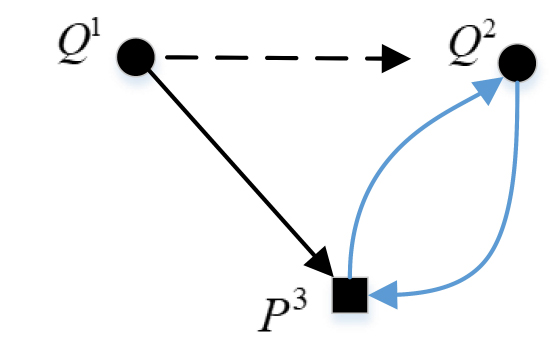
\includegraphics[width=2.0in,height=1.2in]{./figures/decision.jpg}
	\caption{理性决策过程的描述说明}
	\label{fig:chapter07_rational}
\end{figure}

{\em 通过分析算法\textup{\ref{alg:game}}的一些基本操作,给出计算博弈鞍点的计算复杂度。首先,算法在第一轮迭代中搜索攻击者的策略空间$\mathcal{P}$,寻找一个最优的响应策略$P$。其次,针对攻击者策略算法计算一个最优响应策略$Q$,需要搜索防护者的策略空间$\mathcal{Q}$。最后,算法的终止条件保证了极大极小问题的解。鉴于上述分析可知,计算开销随着$\mathcal{P}$和$\mathcal{Q}$的大小而变化。只要策略集合$\mathcal{P}$和$\mathcal{Q}$是有限的,算法计算过程是有效的。
}
\section{实验与分析}\label{sec:chapter06-experiment}
本节中给出所提出隐私保护策略选择方案的实验结果,并给出实验结果的分析。基于Java实现本章中伪代码描述的算法,并部署在安装Windows 10操作系统的个人PC上执行实验程序。实验分析有两个部分组成,首先,\ref{sec:case_study}节给出一个具体的实例分析,随后,\ref{sec_numberic_simulation}节给出数值实验分析结果。
\subsection{实例分析}\label{sec:case_study}

对于字母表$|\mathcal{X}| = |\hat{\mathcal{X}}|=6$的情况,本章假设数据先验分布属于一个确定的概率分布集合,但是不能精确的知道真实的数据分布。为了有一个直观的说明,本章借用文献\mycite{kalantari2018robust}中的分布数据,并在表\ref{tab:chapter07_5}中给出它们的分布律。

\begin{table}[!ht]
	%\scriptsize
    \small
	\caption{$|\mathcal{X}|=6$的概率分布}
	\label{tab:chapter07_5} \centering
	\begin{tabular}{p{1cm}p{1cm}p{1cm}p{1cm}p{1cm}p{1cm}p{1cm}}
		\hline\noalign{\smallskip}
		& $p_{(1)}$ & $p_{(2)}$ & $p_{(3)}$  & $p_{(4)}$ & $p_{(5)}$ & $p_{(6)}$ \\
		\noalign{\smallskip}\hline\noalign{\smallskip}
		$P^{1}$ & 0.7 & 0.15 &0.06 & 0.04 & 0.03 &0.02\\
		$P^{2}$ & 0.15 & 0.7  &0.06 & 0.04 & 0.03  &0.02\\
		$P^{3}$ & 0.06 & 0.15  &0.7 & 0.04 & 0.03  &0.02\\
		$P^{4}$ & 0.04 & 0.15  &0.06 & 0.7 & 0.03  &0.02\\
		\noalign{\smallskip}\hline
	\end{tabular}
\end{table}
更多的,考虑两个等价可替换的$\epsilon=\ln 2$隐私机制,表\ref{tab:chapter07_6}给出两个隐私机制的条件概率分布,其中,$Q^1$是截断$\frac{1}{2}$- 几何机制\cite{ghosh2012universally},$Q^2$是文献\mycite{alvim2011differential}提出的隐私机制。进一步,考虑文献\mycite{kairouz2016extremal}中提出的著名$k$-RR机制,满足对角线概率$e^{\epsilon}/(|\mathcal{X}|-1+e^{\epsilon})$。基于此,$k$-RR提供$\epsilon=\ln 2$差分隐私保护,当且仅当概率密度函数$Q^3$满足
\begin{equation}\nonumber
	Q_{(y|x)}^3 = \begin{cases}
		\frac{e^{\epsilon}}{|\mathcal{X}|-1 +e^{\epsilon}} & \hat{x}=x\\
		\frac{1}{|\mathcal{X}|-1 +e^{\epsilon}} & \hat{x}\neq x
	\end{cases}
	\Rightarrow Q_{(y|x)}^3 = \begin{cases}
		2/7 & \hat{x}=x\\
		1/7 & \hat{x}\neq x
	\end{cases}
\end{equation}

\begin{table*}[htbp]
	%\scriptsize
\small
	\centering
	\caption{$|\mathcal{X}|=6$时提供$\epsilon=\ln2$的等价隐私机制}
	\label{tab:chapter07_6}
	\begin{tabular}{ccccccccccccc}
		\toprule
		\multirow{2}{*}{In/Out} & \multicolumn{6}{c}{$Q^1_{(y|x)}$} & \multicolumn{6}{c}{$Q^2_{(y|x)}$} \\
		\cmidrule(r){2-7} \cmidrule(r){8-13}
		&  $1$      &  $2$   &   $3$ &  $4$      &  $5$   &   $6$
		&  $1$      &  $2$   &   $3$ &  $4$      &  $5$   &   $6$\\
		\midrule
		$1$  &$2/3$  & $1/6$ &$1/12$   & $1/24$  & $1/48$   & $1/48$             &$4/11$  & $2/11$ &$1/11$ & $1/11$ &$1/11$  & $2/11$ \\
		$2$  &$1/3$   &$1/3$  & $1/6$ & $1/12$  & $1/24$  & $1/24$               &$2/11$  & $4/11$ &$2/11$ & $1/11$ &$1/11$  & $1/11$ \\
		$3$ &$1/6$ & $1/6$  & $1/3$  & $1/6$  & $1/12$ & $1/12$                  &$1/11$  & $2/11$ &$4/11$ & $2/11$ &$1/11$  & $1/11$ \\
		$4$ &$1/12$ & $1/12$  & $1/6$  & $1/3$  & $1/6$ & $1/6$                  &$1/11$  & $1/11$ &$2/11$ & $4/11$ &$2/11$  & $1/11$ \\
		$5$  &$1/24$ & $1/24$  & $1/12$  & $1/6$  & $1/3$ & $1/3$                &$1/11$  & $1/11$ &$1/11$ & $2/11$ &$4/11$  & $2/11$ \\
		$6$ &$1/48$ & $1/48$  & $1/24$  & $1/12$  & $1/6$ & $2/3$                &$2/11$  & $1/11$ &$1/11$ & $1/11$ &$2/11$  & $4/11$ \\
		\bottomrule
	\end{tabular}
\end{table*}

上述隐私机制$\{Q^1,Q^2,Q^3\}$是等价的$\ln 2$-隐私机制。为了对这些隐私机制进行比较,假设它们是隐私防护者的所有可能策略。基于这个假设,在此给出以下分析。

基于上述的这些参与者可选行动策略,分析隐私攻击者和防护者的理性策略行为。通过算法\ref{alg:game}求解所对应的博弈模型。作为博弈的解,算法输出一个鞍点$P^1,Q^3$ 和支付量$0.0351$,这个结果意味着互信息隐私泄露将不会超过一个界($0.0351$)。在其它策略组合情况下,隐私防护者将会有动机改变他当前的隐私保护策略。例如,当考虑均匀的先验概率分布,对策博弈的支付量将会是$0.0633$。综合上述情况,这些情况意味着最佳的隐私保护机制和先验分布密切相关。

此外,本章还利用信息论度量方法解决了等价隐私保护机制之间无法比较的问题。例如,考虑均匀的先验概率分布情景,这些隐私机制的互信息隐私泄露是严格有序的,即$Q^1=0.5074 > Q^2=0.2164>Q^3=0.0633$。事实上,互信息隐私泄露的这些数值表达出了隐私防护者对于不同博弈产出的偏好。由此,则可以得到$Q^3 \succ Q^2 \succ Q^1$。这种严格的偏序关系对等价的隐私保护机制提供了一种有效的评估方法。


\subsection{数值分析}\label{sec_numberic_simulation}
为了获得数值实验结果,本文中分别对$|\mathcal{X}|=6$和$|\mathcal{X}=12|$随机的生成$10$个不同的分布。然后,利用随机化响应技术实现隐私保护机制。参考文献\mycite{kairouz2016extremal},实验中设置$\epsilon$参数在$0$到$10$的区间变化,如此可以获得一个隐私保护机制的集合。基于这些随机的数值数据,给出下面的实验分析。

数据先验概率分布和随机生成的不同隐私机制分别为隐私攻击者和隐私防护者的可用策略行动,并在这些数据上执行实验,利用所提出的策略优化选择算法\ref{alg:game}计算隐私保护攻防博弈的鞍点。为了克服随机性的影响,实验中通过归一化的互信息$I(X;\hat{X}/H(X))$比较所有隐私机制的平均性能,也即是隐私支付量。在所提出的隐私攻防博弈模型中,理性的隐私攻击者和隐私防护者偏好于采用获得最大化(最小化)博弈支付的策略。事实上,互信息隐私泄露是隐私预算$\epsilon$的严格单调函数,由此,随着$\epsilon$的增加,归一化的互信息隐私泄露曲线可以被描绘出来。

\begin{figure}[htbp]
\centering
\begin{minipage}[t]{0.48\textwidth}
\centering
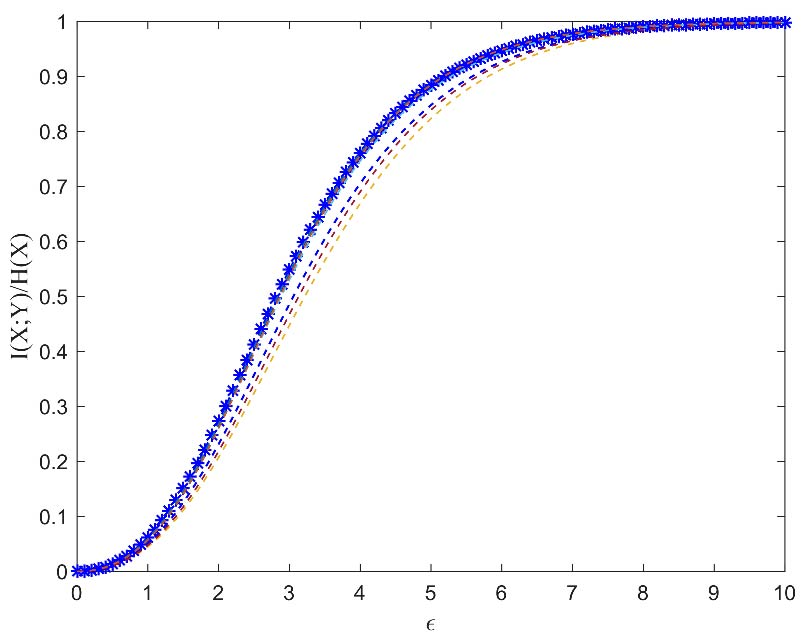
\includegraphics[width=7cm,height=2.0in]{./figures/Fig3.jpg}
\caption{$|\mathcal{X}|=6$时$I(X;\hat{X})/H(X)$}
\label{Fig:chapter06-3}
\end{minipage}
\begin{minipage}[t]{0.48\textwidth}
\centering
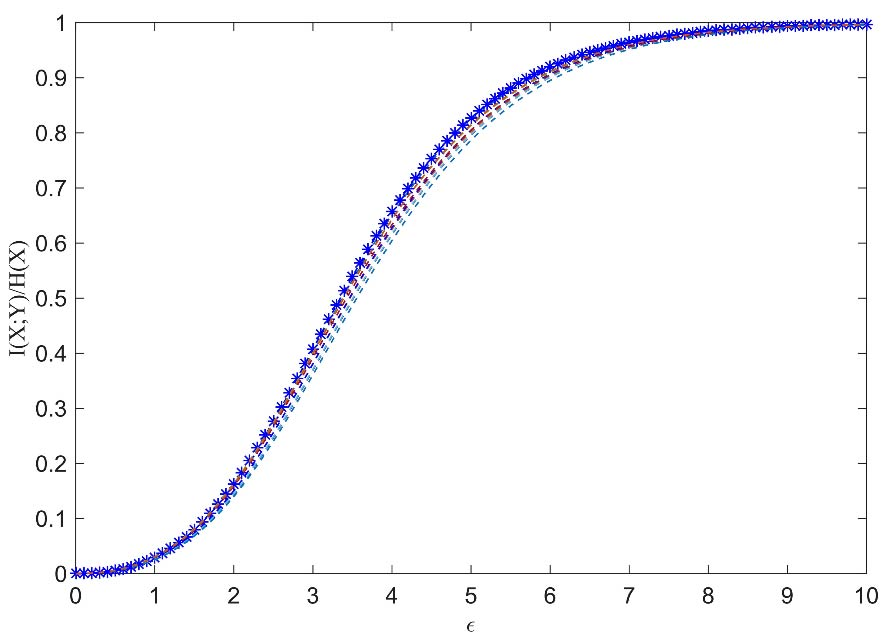
\includegraphics[width=7cm,height=2.0in]{./figures/Fig4.jpg}
\caption{$|\mathcal{X}|=12$时$I(X;\hat{X})/H(X)$}
\label{Fig:chapter06-4}
\end{minipage}
\end{figure}

%\begin{figure*}[htbp]
%	\centering
%		\begin{minipage}[t]{7cm}
%			\centering
%			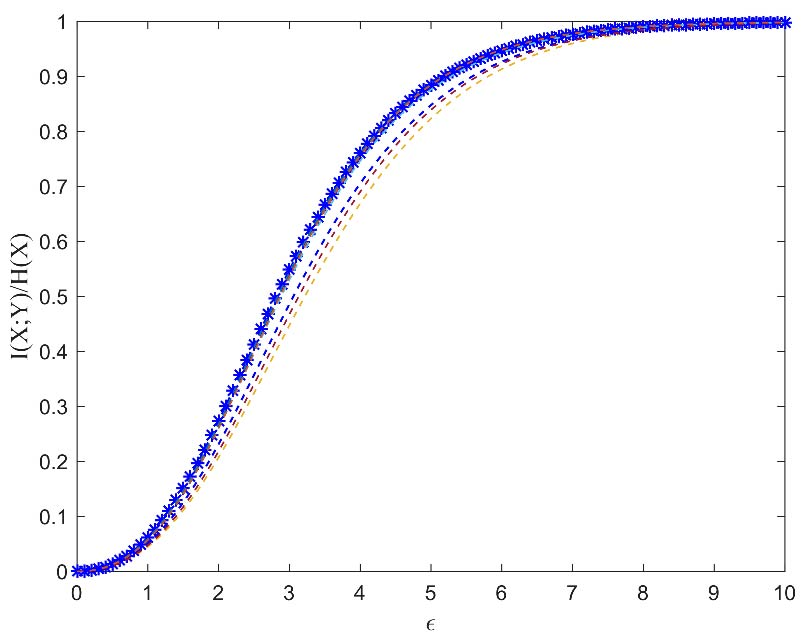
\includegraphics[width=2.5in,height=2.0in]{./figures/Fig3.jpg}
%			\label{Fig:3a}
%		\end{minipage}
%		\begin{minipage}[t]{7cm}
%			\centering
%			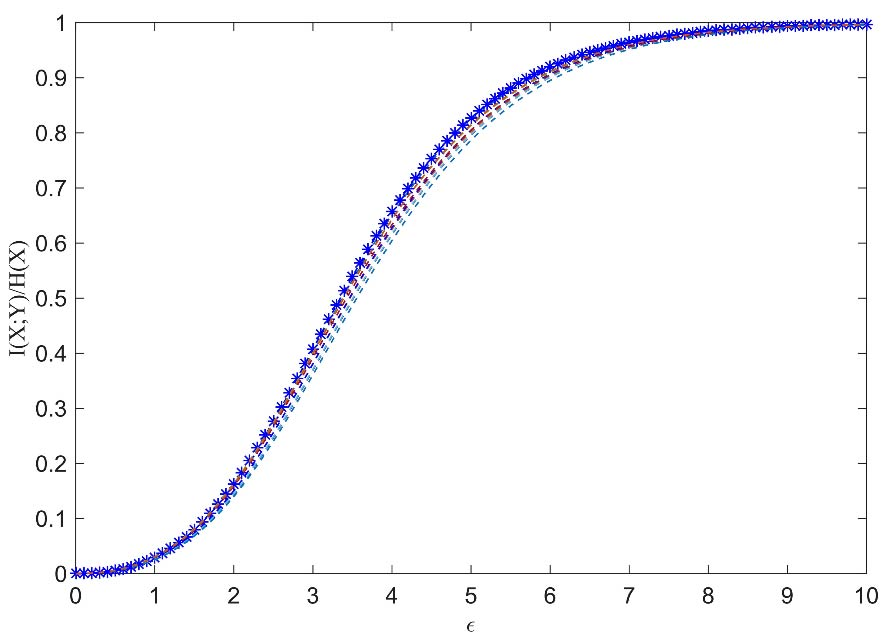
\includegraphics[width=2.5in,height=2.0in]{./figures/Fig4.jpg}
%			\label{Fig:3b}
%		\end{minipage}
%	\centering
%	\caption{隐私机制的归一化$I(X;\hat{X})/H(X)$ 对于随机生成的$10$个分布}
%	\label{fig:numerical simulation}
%\end{figure*}
图~\ref{Fig:chapter06-3}和图~\ref{Fig:chapter06-4}给出了数值实验结果。从图中可以看出,鞍点策略的互信息隐私泄露对于隐私防护者是最差情况的隐私泄露。另外,图~\ref{Fig:chapter06-3}和图~\ref{Fig:chapter06-4}还表明了上述结论对于字母表基数$|\mathcal{X}|$是不敏感的,因为两组实验具有相同的趋势。最差情况下的互信息隐私泄露可以帮助评估隐私泄露风险,选择适当的$\epsilon$参数在隐私容忍的范围内。

\section{本章小结}\label{sec:chapter06-conclusion}

本章针对差分隐私数据收集应用中存在的策略型攻击问题,利用信息论、博弈均衡理论研究了隐私防护者与隐私攻击者的理性策略选择,提出了隐私保护的攻防博弈(PPAD)模型,以实现隐私与数据效用均衡。首先,基于信息论度量方法分析差分隐私保护系统中隐私保护者和攻击者的隐私目标,形式化表述为互信息隐私的极大极小问题。其次,针对上述提出的问题,考虑策略型的隐私攻击者和防护者,提出隐私保护的攻防博弈模型,并具体为二人的零和博弈模型。随后,给出博弈的凹凸性以及均衡分析。进一步,为了求解博弈模型鞍点,设计了策略优化选择算法。最后,通过实验阐述了所提出的方案可以用于比较等价的隐私机制,并阐述了隐私量化是最坏情况下的隐私泄露,也即是,隐私防护者的最大隐私泄露。
